% \documentclass[aip,jcp,preprint,unsortedaddress,a4paper,onecolum]{revtex4-1}
\documentclass[]{tMPH2e}
% \documentclass[aps,pre,twocolumn]{revtex4-1}
% \documentclass[aps,jcp,groupedaddress,twocolumn,unsortedaddress]{revtex4}

% \usepackage[fleqn]{amsmath}
% \usepackage{amssymb,amsthm}
% \usepackage[dvips]{graphicx}
% \usepackage{color}
% \usepackage{tabularx}
% \usepackage{algorithm}
% \usepackage{algorithmic}

\makeatletter
\makeatother


\newtheorem{thm}{Theorem}

\newcommand{\recheck}[1]{{\color{red} #1}}
\newcommand{\redc}[1]{{\color{red} #1}}
\newcommand{\bluec}[1]{{\color{blue} #1}}
\newcommand{\vect}[1]{\textbf{\textit{#1}}}
\newcommand{\dd}{\textsf{d}}
\newcommand{\inv}{\textrm{inv}}


\newcommand{\R}{{\mathbf R}}
\newcommand{\Q}{{\mathbf Q}}
\newcommand{\Z}{{\mathbf Z}}
\newcommand{\N}{{\mathbf N}}
\newcommand{\T}{{\mathbf T}}
\newcommand{\mh}{\mathcal H}
\newcommand{\eps}{\varepsilon}
\newcommand{\ml}{\mathcal L}
\newcommand{\mt}{\mathcal T}
\newcommand{\mo}{\mathcal O}
\newcommand{\mi}{\mathcal I}
\newcommand{\mc}{\mathcal C}
\newcommand{\proj}{\mathit\Pi}
\newcommand{\fwg}{{\mathcal A}}
\newcommand{\cA}{\mathcal A}
\newcommand{\bwg}{{\mathcal B}}
\newcommand{\bsigma}{\boldsymbol\sigma}
\newcommand{\bE}{{\mathbf E}}
\newcommand{\bP}{{\mathbf P}}
\newcommand{\one}{{\mathbf 1}}
\newcommand{\zero}{{\mathbf 0}}

\newcommand{\wrt}{with respect to }


\begin{document}

% \title{Linear response theory for core set identification}
\title{Linear response theory for a system under non-equilibrium conditions}

\author{Han Wang$^{a}$ and Carsten Hartmann$^{a}$ and Christof Sch\"utte$^{a,b}$$^{\ast}$\thanks{$^\ast$Corresponding author. Email: Christof.Schuette@fu-berlin.de}\\\vspace{6pt}$^{a}${\em Institute for Mathematics, Freie Universit\"at Berlin, Germany}\\$^{b}${\em Zuse Institute Berlin (ZIB), Germany}}
  

% \author{Han Wang}
% \author{Carsten Hartmann}
% \affiliation{Institute for Mathematics, Freie Universit\"at Berlin, Germany}
% \author{Christof Sch\"utte}
% \affiliation{Institute for Mathematics, Freie Universit\"at Berlin, Germany}
% \affiliation{Zuse Institute Berlin (ZIB), Germany}
% \affiliation{Institute for Mathematics, Freie Universit\"at Berlin, Germany}

\maketitle

\begin{abstract}
  In this paper, we firstly review standard equilibrium linear response
  theory in the context of molecular dynamics, and then generalize it to systems in nonequilibrium and under a nonequilibrium
  driving. We calculate not only the linear response term, but also
  second order terms for small perturbations to the reference dynamics. Furthermore, we outline how the novel nonequilibirum linear response formula can be used to compute optimal controls of molecular systems for cases in which one wants to steer the system to maximize a certain target expectation value.

\end{abstract}


\section{Introduction}

Standard molecular dynamics simulations are dealing with systems in thermal equilibrium; in this case they are tuned to the canonial or Boltzmann distribution in the sense that either (1) if one starts from this distribution it remains invariant under the dynamics or (2) if one generates a very long trajectory it samples state space with respect this distribution, that is, every possible state of the molecular system under consideration is visited according to the probability given by it.  Obviously, this allows to compute equilibrium expectation values with respect to the  canonical distribution simply be computing long trajectories. 

Often, however, one is interested in knowing about the response of the molecular system to perturbation out of equilibrium. The standard linear response formula allows to answer this question, at least partially. In the standard setting it gives us the first order of the change to an equilibrium expectation value as resulting from the non-equilibrium perturbation. Here, first order means first order in the size of the perturbation. This linear response formula has a long history of extensions and generalizations. In some sense it has become one of the cornerstones of modern statistical physics since it can be related to the fluctuation dissipation theorem (FDT) which roughly states that for appropriate systems in statistical equilibrium, the average response to small external perturbations can be calculated through the knowledge of suitable correlation functions of the unperturbed statistical system. In this sense there the standard linear response theory holds in a  very general sense \cite{Majda} as long as one assumes that the unperturbed system is in equilibrium.
%=Martin Hairer and Andrew J Majda, A simple framework to justify linear response theory, Nonlinearity 23 (2010) 909–922 doi:10.1088/0951-7715/23/4/008

There is an increasing number of articles in the literature that report on applications of molecular dynamics to nonequilibrium settings. There are many generalization to so-called nonequilibrium steady states based on the generality of the FDT, but despite its wide use, the present authors do not know of a linear response formula that applies to fully general nonequilibirium cases. We will provide such a formula for the case that the underlying dynamics can be described by Langevin dynamics. Furthermore, we will even provide a formula for the second order response of a Langevin system in non-equilibrium to a small perturbation.

Instead of applying this theory to a molecular system we will go one step further. We will outline how the novel nonequilibrium linear response formula can be used to compute the optimal control of molecular systems. In optimal control one seeks the optimal way to perturbed a molecular system such that a certain target expectation value (e.g. population of certain states) is maximized under constraints on the energy of the control. In general the control drives the molecular system under control out of equilibrium. Thus, the nonequilibrium linear response formula can be used to find the optimal correction of the present control regarding the expectation value of interest. 

The outline of the article is as follows: First, we will review the derivation of the standard linear response formula for  rather general diffusion processes which include which Langevin dynamics. Next, we will show how to derive first and second order response formulas for the nonequilibrium case and how to apply these formula for the computation of optimal controls. Finally, we will validate the nonequilibrium linear response formula and its use for optimal control for simple test cases. This numerical experiments will also outline that the use of the linear response formula is imperative for numerical efficiency and allows to extend the applicability of linear response theory to stronger perturbations. 


 


\section{Linear response}


In this section, we want to firstly give a simple and formal derivation of the linear response for equilibrium and nonequilibrium systems. To this end we consider a general It\^o stochastic differential equation of the form
\begin{equation}\label{sde}
dX_{t} = (b(X_{t},t) + \eps v_{t})dt +a(X_{t})dB_{t}\,,\quad t\ge 0\,,
\end{equation}
where $X_{t}\in\R^{d}$, $b(\cdot,\cdot)$ is a smooth time-dependent vector field, $a(\cdot)$ a smooth field of $d\times n$ matrices and $B_{t}$ is standard Brownian motion in $\R^{n}$. Here $v_{t}\in\R^{d}$ is any given driving force applied to the system, which in general may depend on $X_{t}$ and $t$; $\eps>0$ is a small parameter. We consider the equilibrium and nonequilibrium case separately. 


  




\subsection{Small perturbations from equilibrium: Langevin dynamics}

For the equilibrium case (see, e.g., \cite{XXX,YYY,ZZZ}), we assume that the infinitesimal generator
\[
\fwg^{\eps} = \fwg_{0} + \eps\fwg_{1}\,, 
\]
with 
\[
\fwg_{0} = \frac{1}{2}aa^{T}\colon\nabla^{2} + b\cdot\nabla\,,\quad \fwg_{1}=v\cdot\nabla 
\]
of (\ref{sde}) has an isolated eigenvalue 0 corresponding to the unique invariant measure of the dynamics for $\eps=0$ and satisfies a spectral gap condition (see, e.g., \cite{stoltz2012}), so that the operator $(\fwg_{0}^{*})^{-1}\fwg_{1}^{*}$ is bounded (on an appropriate domain), where $\cA_{0}^{*}$ and $\cA_{1}^{*}$ denote the formal adjoints in $L^{2}$, e.g., $\cA_{1}^{*}\phi=-\nabla(v \phi)$.  

Specifically, we are interested in the case that (\ref{sde}) has the form of a Langevin equation, in which case  
\begin{equation}\label{eqn:langevin-1}
b = \left(\nabla_{p}H, -\nabla_{q} H - \gamma\nabla_{p}H\right )^{T}\,,\quad a= (\zero,\sigma)^{T}\,,
\end{equation}
where $H\colon\R^{d}\to\R$, $d=2n$ is the Hamiltonian of the system, $\gamma=\gamma^{T}>0$ the positive semi-definite $n\times n$ friction matrix, $\sigma$ constant, satisfying $2\gamma=\beta\sigma\sigma^{T}$ for some $\beta>0$, and we have used the convention $x=(q,p)\in\R^{n}\times\R^{n}$. Under these conditions on friction and noise and some mild growth conditions on the Hamiltonian for large arguments, the unperturbed dynamics has a unique invariant measure with density 
\[
\rho_{0}(q,p) = \frac{1}{Z}e^{-\beta H(q,p)}\,,\quad  Z=\int  e^{-\beta H(q,p)}\,dqdp\,.
\] 
and the above spectral gap condition is met. Now let $f$ be any integrable phase space function and let $\rho^{\eps}=\rho^{\eps}(q,p,t)$ denote the probability density of $X_t=(Q_{t},P_{t})$, the solution to the Langevin equation (\ref{sde})--(\ref{eqn:langevin-1}), assuming that $(Q_{0},P_{0})=(q,p)$ was distributed according to the invariant density $\rho_{0}$. We define the expectation \wrt $\rho^{\eps}$ as 
\[
\bE_{\rho^{\eps}}[f] = \int f \rho^{\eps} \,dqdp\,.
\] 
A classical result (see, e.g., \cite{HairerMaijda08} and the references therein), that is usually derived using a formal expansion of the solution to the Kolmogorov forward or backward equations in powers of $\eps$, now states that 
\begin{equation}\label{lr}
\lim_{\eps\to 0}\frac{\bE_{\rho^{\eps}}[f] - \bE_{\rho^{0}}[f]}{\eps} = \bE_{\rho^{0}}[\cA_{1}\cA_{0}^{-1}(f-\bE_{\rho^{0}}[f])]\,.
\end{equation}

\subsubsection*{Green-Kubo relations} 
For the specific case of the Langevin equation (\ref{sde})--(\ref{eqn:langevin-1}), the general linear response (\ref{lr}) can be recast in form of the better known Green-Kubo formula \cite{MarconiPhysRep,Risken}. Using the formal operator identity 
\[
-\cA_{0}^{-1} g = \int_{0}^{\infty}e^{t\cA_{0}}g \,dt\,,
\]
that can shown to hold for the generator of the Langevin equation under mild conditions (formally for functions $g$ that are orthogonal to the nullspace of $\cA_{0}^{*}$, i.e. functions satisfying $\bE_{\rho_{0}}[g]=0$), we find that 
\begin{equation}\label{GreenKubo}
\lim_{\eps\to 0}\frac{\bE_{\rho^{\eps}}[f] - \bE_{\rho^{0}}[f]}{\eps} = -\beta\int_{0}^{\infty}\bE_{\rho^{0}}[J(Q_{0},P_{0}) (f(Q_{t},P_{t})-\bE_{\rho^{0}}[f])]\,,dt
\end{equation}
in terms of the dissipative flux $J=-v\cdot\nabla H$, where the expectation under the integral is taken over all realizations/path of the unperturbed Langevin equation with initial distribution $\rho^{0}(q,p,0)=\rho_{0}$. In other words: 
\[
\bE_{\rho^{\eps}}[f] \approx \bE_{\rho_{0}}[f] - \eps\beta\int_{0}^{\infty}\bE_{\rho_{0}}[J(Q_{0},P_{0}) (f(Q_{t},P_{t})-\bE_{\rho_{0}}[f])]\,dt.
\]




%%%%%%%%%%%%%%%%%%%%%%%%%%%%%%%%%%%%%%%%%%%%%%%%%%%%%%%%%%%%%%%%%%%%%%%%%%%%%%%%%%%%%%%%%%%%%%%%%%%%%%%%%
%%%%%%%%%%%%%%%%%%%%%%%%%%%%%%%%%%%%%%%%%%%%%%%%%%%%%%%%%%%%%%%%%%%%%%%%%%%%%%%%%%%%%%%%%%%%%%%%%%%%%%%%%

\subsection{Nonequilibrium response theory: controlled Langevin dynamics}

The classical response theory has the limitation that the reference (equilibrium) distribution $\rho_{0}$ must be stationary under the dynamics and is unique. Moreover the validity of the linear approximation relies on a spectral gap condition that is difficult to verify in practice. In particular the perturbation argument does not provide a framework, under which the second and even higher order responses can be easily derived. 

\subsubsection*{Girsanov transformation}

Here we propose an alternative (purely formal) derivation of the linear response result, that is based on a change of drift in the corresponding SDE and which allows for an easy generalization of the above linear response result to nonequilibrium systems. We will briefly review the idea of the change of drift via Girsanov transformations; for details we refer to the textbook~\cite{oksendal2003stochastic}. Now let $x_{t},X_{t}$ be the solutions to the following stochastic differential equations:
\begin{subequations}\label{sde2}
\begin{align}
dx_{t} & = b(x_{t},t)dt + a(x_{t})dB_{t} \label{sde2-1}\\
dX_{t} & = (b(X_{t},t) + \eps v_{t})dt +a(X_{t})dB_{t} \label{sde2-2}
\end{align}
\end{subequations}
for $0\le t\le T$ and with fixed initial conditions
\[
x_{0} = X_{0} = x\,,
\]
Suppose that there exists a auxiliary stochastic process $\xi_{t}\in\R^{m}$ such that 
\begin{equation}\label{xi}
a(X_{t})\xi_{t} = v_{t}\,,
\end{equation}
The auxiliary variable $\xi$ will be called \emph{control variable}. We define  
\[
W_{t} = \eps\int_{0}^{t}\xi_{s}\,ds + B_{t}\,,\quad 0\le t\le T\,,
\]
which allows us to express (\ref{sde2-2}) by
\begin{equation}\label{sde2-3}
dX_{t} = b(X_{t},t)dt +a(X_{t})dW_{t} 
\end{equation}
It follows from the Girsanov theorem \cite[Thm.~8.6.8]{oksendal2003}, sometimes also called \emph{Cameron-Martin-Girsanov theorem} \cite{a}, that $W_{t}$ is again a Brownian motion under a new probability measure that has a density \wrt the Gaussian probability measure that is generated by the Brownian motion $B_{t}$. Specifically, let $\nu$ denote the law of the Brownian motion $B_{t}$ and define a new probability measure $\mu$ on the space of continuous trajectories by 
\[
d\mu=M_{T}d\nu
\]
with 
\begin{equation}\label{likelihood}
M_{t} = \exp\left(-\eps\int_{0}^{t}\xi_{s}\cdot dB_{s} - \frac{\eps^{2}}{2}\int_{0}^{t}|\xi_{s}|^{2}ds\right)\,,\quad 0\le t\le T\,.
\end{equation}
Technical details aside, the Girsanov theorem implies that $W_{t}$  for any function $f=f(\{X_{t}\}_{0\le t\le T})$ that is integrable \wrt $\nu$, we have the identity
\[
\bE_{\nu}[f] := \int f(\{X_{t}\}_{0\le t\le T})\, d\nu = \int f(\{X_{t}\}_{0\le t\le T}) \frac{d\nu}{d\mu}\,d\mu =: \bE_{\mu}[M^{-1}_{T}f]\,.
\]
where 
\[
M_{T}^{-1} = \exp\left(\eps\int_{0}^{T}\xi_{s}\cdot dW_{s} - \frac{\eps^{2}}{2}\int_{0}^{T}|\xi_{s}|^{2}ds\right)\,.
\]
is the density of $\nu$ relative to $\mu$. 



Linearization of $M_{T}^{-1}$ about $\eps=0$, assuming that the control has bounded variance, yields the alternative linear response formula 
\begin{equation}\label{lr-alt}
\lim_{\eps\to 0}\frac{\bE_{\nu}[f] + \bE_{\mu}[f]}{\eps} = \bE_{\mu}\left[f(\{X_{t}\}_{0\le t\le T})\int_{0}^{T}\xi_{s}\cdot dW_{s} \right]\,,
\end{equation}
where $X_{t}$ is the solution (\ref{sde2-3}). Note that this is the unperturbed nonequilibrium dynamics, because $W_{t}$ is a standard Brownian motion under $\mu$, and the expectation is over all realizations of (\ref{sde2-3}) starting from either any given initial condition $X_{0}=x$ or an arbitrary initial distribution. On the other hand, $X_{t}$ under $\nu$ corresponds to the perturbed dynamics, which should become clear upon comparing equations (\ref{sde2-2}) and (\ref{sde2-3}). Further note that $f$ and $W_{t}$ are not independent, hence the expectation on the right hand side of the equation is not zero in general. 


\paragraph*{Remark.} A quick-and-dirty derivation of the above change-of-measure formula can be easily obtained, if the noise covariance $a(\cdot)a(\cdot)^{T}$ has full rank almost everywhere with bounded inverse. Then, using Euler's method for (\ref{sde2}), it follows that (\ref{likelihood}) is basically the likelihood ratio between the time-discrete path densities of (\ref{sde2-2}) and (\ref{sde2-1}).    

\paragraph*{Remark.} By formally expanding $M^{-1}_T$ up to second order we get an analogous second order response formula: 
\begin{equation}\label{2nd}
\bE_{\nu}[f] \approx \bE_{\mu}[f] + \eps \bE_{\mu}\left[f\int_{0}^{T}\xi_{s}\cdot dW_{s} \right] +\frac{\eps^{2}}{2} \bE_{\mu}\left[f\left\{\left(\int_{0}^{T}\xi_{s}\cdot dW_{s}\right)^2 -\int_0^T |\xi_s|^2\,ds\right\} \right]
\end{equation}
 





\subsubsection*{Nonequilibrium Langevin equation}

We now link our previous considerations with the previous case and consider a non-equilibrium Langevin equation. Specifically, we add a non-gradient perturbation to the Langevin equation 
\begin{equation}\label{eqn:langevin-1b}
b = \left(\nabla_{p}H, -\nabla_{q} H - \gamma\nabla_{p}H  + D(q) u \right)^{T}\,,\quad a= (\zero,\sigma)^{T}\,,
\end{equation}
where $u\in\R^{n}$ is some control variable and $D(\cdot)\in\R^{n\times n}$ satisfies the Fredholm alternative $\mathrm{range}(D(\cdot))\perp \mathrm{ker}(\sigma^{T})$, where $\mathrm{ker}(\sigma^T)$ denotes the kernel of $\sigma^T$. As we are interested in small perturbation $\delta u$ in the controls $u$, it is convenient to further specify what $v$ in (\ref{sde2}) is. Specifically, we assume that $v$ is of the form 
\begin{equation}\label{eqn:langevin-1c}
v = (\zero, D(q)\,\delta u)
\end{equation}
so that equation (\ref{xi}) that determines the change of measure in terms of the auxiliary control variable $\xi$ (and thus the linear response) reads 
\[
\sigma \xi_{t} = D(Q_{t})\,\delta u_{t}\,.
\]
To be more explicit, the equation we are considering has the form
\begin{equation}\label{eqn:langevin-1d}
\begin{aligned}
dQ_t & =  \nabla_p H(Q_t,P_t)\\
dP_t & =  -\nabla_q H(Q_t,P_t) - \gamma \nabla_p H(Q_t,P_t) + D(Q_t)\,(u_t+\eps \delta u_t)+\sigma dB_t,
\end{aligned}
\end{equation}
so that $X_t$ from above now is $(Q_t,P_t)$ and $x_t=(q_t,p_t)$ from above is the solution of our last equation for $\eps=0$.

The equation is solvable by the requirement  $\mathrm{range}(D(\cdot))\perp \mathrm{ker}(\sigma^{T})$, which, if $\sigma$ has full rank, means that $D(\cdot)$ must be invertible almost everywhere. Hence the linear response formula (\ref{lr-alt})  becomes
\begin{equation}\label{lr-alt2}
\lim_{\eps\to 0}\frac{\bE_{\nu}[f] - \bE_{\mu}[f]}{\eps} =  \bE_{\mu}\left[f(\{(Q_{t},P_{t})_{0\le t\le T}\})\int_{0}^{T}(\sigma^{-1}D(Q_{s})\,\delta u_{s})\cdot dW_{s} \right]\,
\end{equation}
or, in other words: 
\begin{equation}\label{eqn:neq-response}
\bE_{\nu}[f] \approx \bE_{\mu}[f] + \eps\bE_{\mu}\left[f(\{Q_{t},P_{t}\}_{0\le t\le T})\int_{0}^{T}(\sigma^{-1}D(Q_{s})\,\delta u_{s})\cdot dW_{s} \right]\,.
\end{equation}
Here, as before, the expectation on the right is over all realizations of (\ref{eqn:langevin-1d}) for $\eps=0$ with arbitrary initial conditions (fixed or distributed); see also the remark below on the choice of initial conditions. 






\paragraph*{Remark.} Some comments on the above result are in order:
\begin{itemize}

\item[(i)] The rightmost term in \eqref{eqn:neq-response} is the linear 
  response to the reference non-equilibrium process (driven by $u_t$ with $\eps=0$). From (\ref{2nd}) we can also get the second order response term. The latter is bounded by the assumption that the controls have bounded second moment.  

\item[(ii)] In the above derivation, we have tacitly assumes that the reference and the perturbed non-equilibrium processes start from the same initial value or
  have the same initial distribution. For fixed initial values (i.e.~points) this assumption cannot be relaxed (because otherwise $dP/dQ$ does not exist). For distributed initial values, however, there is no problem for the unperturbed and perturbed dynamics to have different initial distribution as long as both distributions are strictly positive almost everywhere. In this case one can apply a similar reweighing approach between the initial distribution as we used it for the trajectory ensemble.  

\item[(iii)] If one wants to calculate the same expectation value for a family of non-equilibrium perturbations $\delta u_t$ then 
one does not need to repeat the calculations of \eqref{eqn:neq-response} for every member of the family. 
  If it is possible to
  express different $\delta u_t$ in the same basis, then the responses must only be
  calculated for the single basis functions. Then with a linear combination of the responses on basis functions, one can derive
  the responses for the whole family. This feature will be used below when discussion optimal control as an application of the linear response formula. 
  

\end{itemize}




%%%%%%%%%%%%%%%%%%%%%%%%%%%%%%%%%%%%%%%%%%%%%%%%%%%%%%%%%%%%%%%%%%%%%%%%%%%%%%%%%%%%%%%%%%%%%%%%%%%%%%%%%
%%%%%%%%%%%%%%%%%%%%%%%%%%%%%%%%%%%%%%%%%%%%%%%%%%%%%%%%%%%%%%%%%%%%%%%%%%%%%%%%%%%%%%%%%%%%%%%%%%%%%%%%%

\section{Application of the nonequilibrium response formula: optimal control}

Let us remain in the setting of the last section and assume that we are interested in a finite dimensional family of forcings
\[
\mathcal{F}=\{F_e(t)=\sum_{k=1}^N a_k \Phi_k(t)\},
\]
with explicitly given basis functions $\Phi_k$, $k=1,\ldots,N$.
We are interested in computing the gradient of the expectation value at time $T$ of the observable $\mathcal{O}$ wrt the coefficient vector $(a_k)_{k=1,\ldots,N}$ in the point $F_e(t)=\sum_{k=1}^N a_k \Phi_k(t)$. From Eq. (\ref{eqn:neq-response}) we get with $\Delta F_e(t)=\Phi_k(t)$:
\[
\frac{\partial O(T)}{\partial a_j} = \lim_{\eps\to 0}\frac{1}{\eps}( O_\eps(T) -
  O_0(T))=\big\langle O[\vect X_s]\cdot G_j[\vect X_s]\big\rangle_{0,T},
\]
where $X_t$ and $O_0$ are paths and expectation value wrt. the dynamics \eqref{eqn:langevin-1b}--\eqref{eqn:langevin-2b} with $F_e(t)=\sum_{k=1}^N a_k \Phi_k(t)$ and $\eps=0$, and
\[
G_j[\vect X_t]
  = \frac{1}\sigma\int_0^t
  \Phi_j(s)\,\vect D(\vect q_s)\cdot\dd\vect W_s. 
\]
That is, we can compute all derivatives $\partial O(T)/\partial a_j$ from just one ensemble of paths of $X_t$. 

Now we consider the optimization problem
\[
O_{max}(T) = \max_{F_e\in \mathcal{F}} O[F_e](T),
\]
where $O[F](T)$ is the expectation value of the path observable $\mathcal{O}$ that results from \eqref{eqn:langevin-1b}--\eqref{eqn:langevin-2b} with $F_e=F$ and $\eps=0$.
With the gradient being computed one can solve the optimization problem by means of gradient descent in coefficient space,
\[
a^{(i+1)}=a^{(i)} -\gamma \frac{\partial O(T)}{\partial a}.
\]

%%%%%%%%%%%%%%%%%%%%%%%%%%%%%%%%%%%%%%%%%%%%%%%%%%%%%%%%%%%%%%%%%%%%%%%%%%%%%%%%%%%%%%%%%%%%%%%%%%%%%%%%%
%%%%%%%%%%%%%%%%%%%%%%%%%%%%%%%%%%%%%%%%%%%%%%%%%%%%%%%%%%%%%%%%%%%%%%%%%%%%%%%%%%%%%%%%%%%%%%%%%%%%%%%%%

\section{Numerical tests}

\subsection{The metastability of a single-well potential}

\begin{figure}
  \centering
  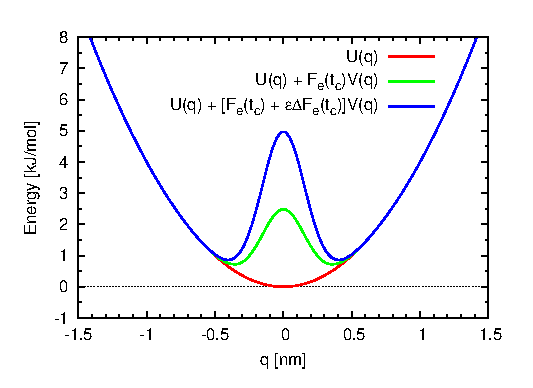
\includegraphics[width=0.4\textwidth]{figs/fig-split-pot.eps}
  \caption{The single-well potential with splitting splitting drving
    force at time $T = 20$ ps.  Since the drving force is
    conservative ($ D( q) = -\nabla_{q}V( q)$),
    we plot the non-equilibrium drving energy of the system.  The red,
    green and blue lines are the potential energy without
    non-equilibrium driving, with non-equilibrium driving and
    the non-equilibrium driving perturbed by $\eps\delta u(t)$,
    respectively.  }
  \label{fig:tmp4}
\end{figure}

We use the idea of non-equilibrium linear response to investigate the
nonequilibrium phase space probability density distribution, denoted by $f(q, p, t)$, of a one-dimensional model system: one particle in a
splitting single-well potential.  For convenience, we let the mass of
the particle to be 1~\textsf{amu}, and the friction coefficient to be
$1\,\textsf{ps}^{-1}$.
The temperature is the
room temperature $300\ \textsf{K}$, $k_BT = 2.48$~\textsf{kJ/mol}.
The unperturbed Hamiltonian of the system is
given by:
\begin{align}
  \mh ( p,  q) = \frac 12  p^2 + U( q) 
\end{align}
with potential
\begin{align}
  U( q) = \frac12\,k\, q^2 
\end{align}
Here $k = 8$~$\textsf{kJ} / (\textsf{mol nm}^2)$.
See the red line in Fig.~\ref{fig:tmp4} for the  potential $U$.
%$\textsf{kJ} / (\textsf{mol nm}^4)}$
The non-equilibrium driving $ D$ is given by a conservative force:
\begin{align}
   D( q) = -\nabla_{ q} V( q) 
\end{align}
where the driving potential $V( q)$ has a Gaussian profile:
\begin{align}
  V( q) = \frac{1}{\sqrt{2\pi \sigma^2}}
  \exp\Big\{-\frac{ q^2}{2\sigma^2}\Big\}
\end{align}
we use $\sigma = 0.16$~\textsf{nm}.  The strength of non-equilibrium
driving $u(t)$ is set to be linearly growing, i.e. $ u(t) = k_e\cdot t/T$,
where $k_e$ is a unitless constant.
We
consider the perturbation to the system given by $\eps\delta u(t) = \eps \cdot t/T$.
We consider the following parameters: end time $T = 20$~\textsf{ps}, 
$k_e = 1$ and $\eps = 1$, see Fig.~\ref{fig:tmp4}
for the non-equilibrium driving potential and perturbed
potential at time $t = T$. The initial distribution $f(q, p, 0)$ is set to
be equilibrium distribution of the unperturbed system.

\begin{figure}
  \centering
  \includegraphics[width=0.95\textwidth]
  {figs/fig-split-str2-2d-distrib-no2nd.eps}
  \caption{ The plot of $ f(q,p,t)$ in the phase
    space under perturbed non-equilibrium driving. From left to right the columns present results at time $t =
    0$, 5, 10 and 20~\textsf{ps}.  The 1st row: the brute force
    non-equilibrium simulation. The 2nd row: the results of
    traditional equilibrium linear response theory. In this case we
    effectivly consider an equilibrium system free of driving, and the perturbation $\eps$ is set to 2.  The 3rd row: the
    non-equilibrium linear response result.  }
  \label{fig:tmp6}
\end{figure}

Fig.~\ref{fig:tmp6} presents the numerical results of the phase space probability distribution for the splitting
single-well potential. From left to right the four rows presents the
distribution of the system at time $t = 0$, 5, 10 and 20~\textsf{ps}. The first
row presents the brute force non-equilibrium simulation.  It is clear
that at the beginning, the distribution has only one peak,
i.e. arount $q = 0$ and $p = 0$. As the time evolves, an energy barrier develops
in the center of the simulation region, therefore, the single peak
splits into two equally sized peaks.  In the end, the two
peaks are entirly seperated.  This brute force non-equilibrium
simulation serves as the precise result that the response theory
should compare with. The second row shows the result of the
traditional equilibrium linear response theory.  Please notice that in
this case, since the reference simulation is in equilibrium, so 
the effective perturbation is of strength $\eps = 2$.  At $t \leq
15$~\textsf{ps}, the accuracy of the equilibrium linear response is
perfect. At $t =
20$~\textsf{ps}, magnitude of the peaks are relatively too strong,
and the gap between them is actually negative.
Since the probability distribution is always positive, the
numerical solution of the equilibrium linear response is qualitatively wrong.
The poor accuracy is due to the fact that the strength of perturbation is no
longer small so that the preliminary assumption of the reponse theory
is not well fulfilled.  On the third row of Fig.~\ref{fig:tmp6},
we present the linear response starting from a non-equilibrium driving
of $u(t)$.  The numerical results is satisfactorily consistent with
the brute force non-equilibrium simulation, because the perturbation
($\eps = 1$) is so small that the linear perturbation theory achieves
good accuracy.

% Fig.~\ref{fig:tmp6} presents the numerical results of perturbation $\eps =
% 2$.  Only with a linear response calculated from the equilibrium
% simulation (2nd row), the stability of the two new core sets are too
% strong, and the unstable region between them is over estimated, comparing with
% the brute force simulation presented on the first row.
% We present the  second order response results on the 3rd row, which is
% also calculated from the equilibrium simulation. In this case, the statistical
% error is too large, so that
% the profile of $\mt_\tau f$ is indeed too noisy to draw any useful information.
















% \subsection{The tilting double-well potential}


% We test the idea firstly by a one-dimensional model system: one particle in a
% tilting double-well potential. For convenience, we let the mass of the
% particle to be 1~\textsf{amu},
% and the friction coefficient to be $1\,\textsf{ps}^{-1}$.
% The unperturbed
% Hamiltonian of the system is given by:
% \begin{align}
%   \mh ( p,  q) = \frac 12  p^2 + U( q) 
% \end{align}
% with potential
% \begin{align}
%   U( q) = \frac12 k ( q^2 - a^2)^2
% \end{align}
% Here $k = 8$~$\textsf{kJ} / (\textsf{mol nm}^4)$, and $ a = 1\ \textsf{nm}$.
% At room temperature $300\ \textsf{K}$, $k_BT = 2.48$~\textsf{kJ/mol}.
% The red line in Fig.~\ref{fig:tmp1} presents the unperturbed potential.
% %$\textsf{kJ} / (\textsf{mol nm}^4)}$
% The perturbation is given by
% \begin{align}
%    D( q) = -\nabla_{ q} V( q) = 1
% \end{align}
% Here $V( q) = - q$   effectively tilts the original
% potential $U( q)$ (see the gree and blue lines in Fig.~\ref{fig:tmp1}).
% The strength of $u(t)$ is
% set to be $k_e$, when the time $t$ is larger than some warm-up time $t_c$.
% When $t \leq t_c$, the strength of $u(t)$ is linearly growing,
% i.e. $ u(t) = k_e\cdot t/t_c$.
% We use the value $t_c = 20$~\textsf{ps}, so that the perturbation increases slow
% enough: the typical decaying time scale of the correlation function
% in~\eqref{eqn:eq-lr} is roughly 3~\textsf{ps}.
% We choose $\tau = 1$~\textsf{ps}, and
% % We choose $\mt_\alpha$
% % to be the propagator of the Langevin dynamics at temperature $150$
% % \textsf{K} with $\alpha = 1$ \textsf{ps}.
% consider the stability of the
% distribution $f( x, t)$ at time $t$: $\Delta\mt_\tau f( x, t)$.
% The larger
% this value, the more stable the core sets are.

% See Fig.~\ref{fig:tmp2} and \ref{fig:tmp3} for numerical result.  Both
% the results of the brute-force non-equilibrium simulation
% and that of the response theory are presented.
% In Fig.~\ref{fig:tmp2},
% the good agreement between the brute-force (1st row)
% and the linear response result (2nd row) indicates that $\eps = 2$ is
% indeed a relatively small perturbation to the equilibrium.
% In the third row of Fig.~\ref{fig:tmp2},
% the second order response is considered. We do not see any
% substantial improvement of the result by including this higher order term,
% because the
% driving force to the system is small,
% and the linear term is anyway a good approximation.

% In Fig.~\ref{fig:tmp3}, as the
% perturbation grows stronger, the left well becomes less stable, while
% the right well becomes more stable.  When the perturbation is as strong as
% $\eps = 4$, the linear response result (2nd row) is no
% longer precise:
% At $t\geq 20$ \textsf{ps}, the left well basically
% disappears, however, the linear response calculation presents
% artificial structure (that is a small artificial
% stable region accompanied by a small unstable region)
% at the position of the left well.
% The second order response (3rd row) improves the accuracy a little, 
% however, it also includes artificial finer-grained oscillation in the profile.
% At the same time, the numerical uncertainty is higher, so the figure
% looks noisy.
% In the 4th row of Fig.~\ref{fig:tmp3}, we present the linear response result
% that calculate from 
% a intermediate
% non-equilibrium simulation with driving force of $k_e = 2$.
% Notice that the reference simulation in this case is also a
% non-equilibrium simulation, so the effective strength of perturbation
% is reduced to $\eps = 2$. According to Fig.~\ref{fig:tmp1}, this can be
% considered as a small perturbation.
% A substantial improvement is achieved: the profile
% is correctly calculated, and the statistical error is small.

% % the 1st order result of the
% % response formula~\eqref{eqn:pert-approx-1} and
% % \eqref{eqn:pert-approx-2}, with
% % respect to the reference state $F_e^{\textrm{max}} = 2$. The result
% % is impressively improved compared with the linear response with respect to the
% % equilibrium state.




\subsection{Optimal tilting of a double-well potential}
\begin{figure}
  \centering
  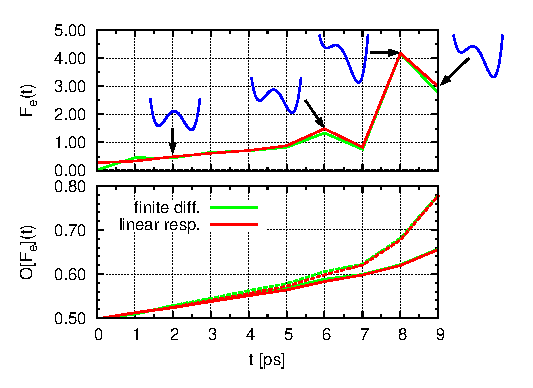
\includegraphics[]{figs/fig-ctr-stat-2.eps}
  \caption{The optimal forcing.  In this plot, $T=20$ ps.  The red
    color indicates $\eta = 0.01$ and the green color indicates $\eta
    = 0.05$.  In the upper plot, the solid lines present the magnitude
    of the control $F_e(t)$, which is calculated on a family of
    piecewise linear ansatz functions. The time interval of a linear
    piece is 1 ps.  The blue insertions show the shape of the
    non-equilibrium driving potential $U( q) + F_e(t)V(
    q)$ at time indicated by the black arrow.  In the lower plot, the
    dashed lines display the value of $P( X_t)$ as the time
    evolves.  The solid lines present $O[F_e](t)$.  }\label{fig:tmp7}
\end{figure}

In this section, we consider the following double well potential:
\begin{align}
  U( q) = \frac12 k ( q^2 - a^2)^2
\end{align}
Here $k = 8$~$\textsf{kJ} / (\textsf{mol nm}^4)$, and $ a = 1\
\textsf{nm}$.  See the leftmost blue insertion of Fig.~\ref{fig:tmp7} for
the shape of the potential.
%$\textsf{kJ} / (\textsf{mol nm}^4)}$
The perturbation is given by a conservative tilting to $U( q)$:
\begin{align}
   D( q) = -\nabla_{ q} V( q) = 1
\end{align}
Here $V( q) = - q$. We want to
optimally design the tilting such that the probability
of being in the right well is as high as possible 
at the end time of the process. That is equal to consider the 
the following optimal forcing problem:
\begin{align}
  O_{\max}(T)& = \max_{F_e\in\mathcal F} O[F_e](T) 
\end{align}
with
\begin{align}
  O[F_e](T) &= P( X_T) -
  \eta\,
  \big\langle \int_0^T\vert F_e(t) D( q)\vert^2\, dt\,
  \big\rangle
\end{align}
where $P( X_T)$ is probability of the end point of the trajectory
$ X_T$ being in the right well.  It is
clear that for an unbiased double-well, $P( X_T)$
is 0.5.  The integral is the ``cost'' of the control and $\eta$ is a
positive constant that indicates the relative magnitude of the
cost. We consider the ansatz function family $\mathcal F$ of piecewise
linear functions on $[0, T]$.

Fig.~\ref{fig:tmp7} presents the numerical result. The magnitude of
control $F_e(t)$ is shown in the upper plot, and the value of
optimization target $O[F_e](T)$ and the value of $P( X_T)$ are
given in the lower plot by the solid and dashed lines, respectively.
The plot shows that with a smaller $\eta$ (the relative magnitude of
the cost of the control is smaller), a stronger control is calculated
from the optimization, and the optimized value of $O[F_e](T)$ and
$P( X_T)$ are bigger, which means the end position of $ X_t$
is more biased towards the right well. This observation is consistent
with intuition.  When $t<10$~ps, the magnitude of the control is
almost 0.  Near the end time $T$, the magnitude of the control firstly
quickly goes up, and then falls down a little bit.  This implies some
interesting information.  If the system were able to immediately relax
to its instantaneous equilibrium state (sometimes called
quasi-equilibrium), the population in the right well (dashed lines in
Fig.~\ref{fig:tmp7}) would immediately go down, as the control
decreases.  The fact that this does not happen, indicates that the
speed of changing the control is relatively faster that the internal
time scale of the system, so the system does not have enough time to
fully relax itself. Therefore, the observed phenomenon is truly
non-equilibrium, and our non-equilibrium linear response theory is a
tool that facilitates the investigation of this optimal forcing
problem in the non-equilibrium setting.  Intuitively, one concludes
that as the control goes up, the population in the right well actually
does not have enough time to go as high as it could be, so when the
control decreases, it continues going up rather than following the
decreasing control.




\section{Conclusions and Remarks}

We derived  first and second order response formulas for molecular dynamics (driven Langevin dynamics) starting from general nonequilibrium distributions. For the special case of the initial distribution being the equilibrium distribution of the unperturbed dynamics, the novel linear response formula siimplifies to the well-known standard formula. We validated the novel formula in numerical experiments in comparison to brute-force nonequilibrium simulations. There, we demonstrated that the novel linear response formula allows to extend the algorithmic use of linear response theory to significantly stronger perturbutions of the system since it permits intermediate steps based on partially propagated nonequilibrium distributions. 

By means of this theory we outlined how to use the novel linear response formula for the computation of optimal controls in molecular dynamics where one desires to find the optimal perturbation/control that maximizes a target functional, that is, a certain expectation value (like the population of a certain region of state space) under a constraint on the energy used in the perturbation. Application of the novel nonequilibrium theory allows to compute the gradient of the target functional by computing expectation values \emph{only} for the dynamics at hand which permits efficient application of standard optimization techniques. We illustrated this technique in application to a simple test case and validated it in comparison to brute force optimization.  











\bibliography{ref}{}
\bibliographystyle{tMPH}





\end{document}